\documentclass[10pt,a4paper]{article}
\usepackage{tocloft}
\usepackage{commons/course}


% Define colors for syntax highlighting
\definecolor{keywordstyle}{rgb}{0.0, 0.4, 0.8} % A bluer shade
\definecolor{stringstyle}{rgb}{0.9, 0.17, 0.31} % amaranth
\definecolor{commentstyle}{rgb}{0.1, 0.6, 0.2} % green
\definecolor{numberstyle}{rgb}{0.4, 0.4, 0.4} % gray
\definecolor{backgroundcolor}{rgb}{0.94, 0.97, 1.0} % aliceblue

% Define the Python-like language for syntax highlighting
\lstdefinelanguage{PythonLike}{
	morekeywords={mov, add, sub, cmp, jmp , lw , addi,sw,bne},
	sensitive=false,
	morecomment=[l]{;},
	morestring=[b]",
}

% Set the style for Python-like code
\lstset{
	language=PythonLike,
	basicstyle=\ttfamily\small,
	keywordstyle=\color{keywordstyle},
	stringstyle=\color{stringstyle},
	commentstyle=\color{commentstyle},
	numbers=left,
	numberstyle=\tiny\color{numberstyle},
	stepnumber=1,
	numbersep=5pt,
	keepspaces=true,
	tabsize=4,
	showspaces=false,
	showstringspaces=false,
	showtabs=false,
	breaklines=true,
	breakatwhitespace=false,
	frame=single,
	backgroundcolor=\color{backgroundcolor},
}

\newlistof{listofproblems}{lop}{\normalsize فهرست مطالب}
\newcommand{\addproblem}[1]{\addcontentsline{lop}{listofproblems}{\protect\numberline{}#1}}


\begin{document}


\سربرگ{گروه شماره ۱ : مهدی محمدی (400105239) - ملیکا علیزاده (401106255) - معین آعلی (401105561)}{}{}{استاد: دکتر بردیا صفائی}

\section*{گزارش آزمایش شماره‌ی 4}

\listoflistofproblems

\bigskip
\bigskip
\hrule


\subsectionaddtolist{طراحی سناریوی اول}

ابتدا طبق ویدیو سناریو داده‌شده را با اجزای آن طراحی می‌کنیم. برای اینکار پس از انتخاب اجزا از منوی پایین و قرار دادن آنها در صفحه، با استفاده از کابل \lr{‫‪cooper straight-through‬‬‬}  به هم وصل میکنیم. به اینصورت که ابتدا کامپیوتر اول را به سوئیچ اول و بعد کامپیوتر دوم را به سوئیچ دوم وصل می‌کنیم. در این اتصال از درگاه \lr{FastEthernet0/1} و \lr{FastEthernet0} استفاده می‌کنیم.
\\
برای اتصال \lr{router0}، روی آن کلیک کرده و در تنظیمات physical آن را خاموش می‌کنیم و بعد از منوی سمت چپ ماژول \lr{NM-2FE2W} را به آن اضافه می‌کنیم. در نهایت آن را روشن می‌کنیم. حال با استفاده از درگاه‌های \lr{Fast Interface}، \lr{router0} را به سوئیچ‌ها وصل می‌کنیم.
\begin{figure}[h]
    \centering
    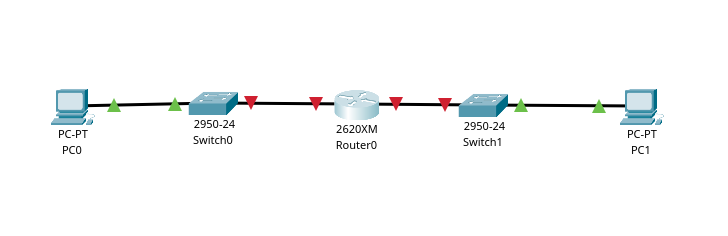
\includegraphics[width=1\textwidth]{img/1.png}
\end{figure}
\begin{figure}[h]
    \centering
    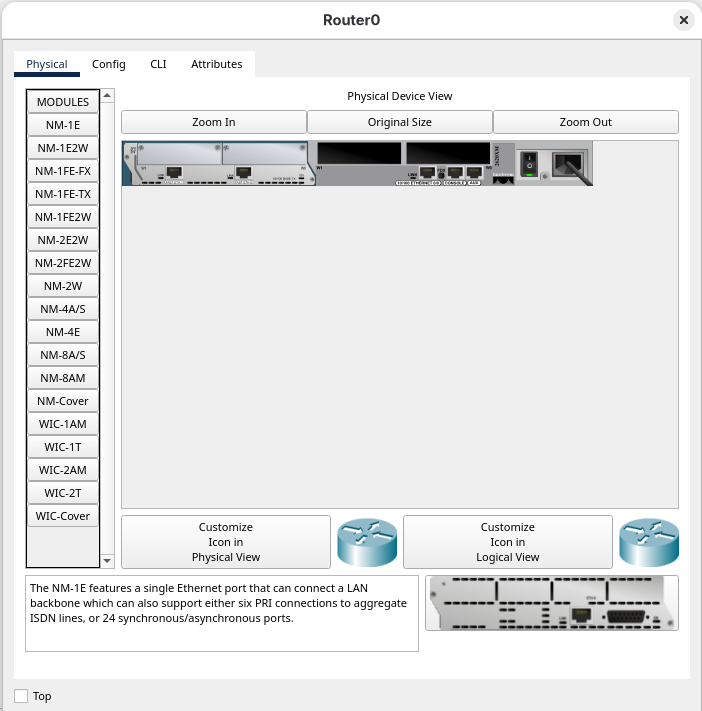
\includegraphics[width=1\textwidth]{img/2.png}
\end{figure}
\clearpage
در ادامه باید IP مسیریاب را تنظیم کنیم. پس با کلید بر روی مسیریاب و در بخش \lr{config}، \lr{FastEthernet1/x} را به صورت زیر پیکربندی می‌کنیم. پس از مشخص کردن مقدار \lr{IPv4} و \lr{subnetmask} مقدار \lr{Port status} را به on تغییر می‌دهیم.
\begin{figure}[h]
    \centering
    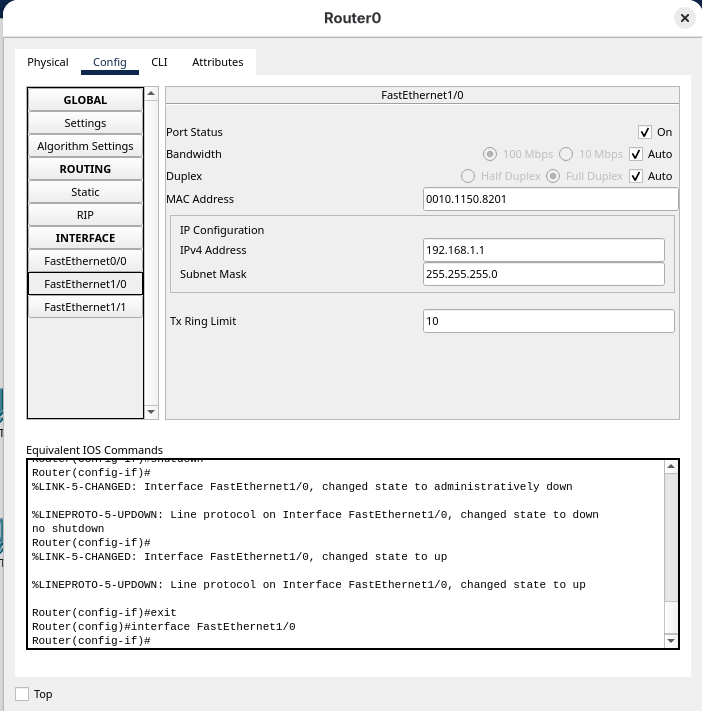
\includegraphics[width=1\textwidth]{img/3.png}
\end{figure}
\begin{figure}[h]
    \centering
    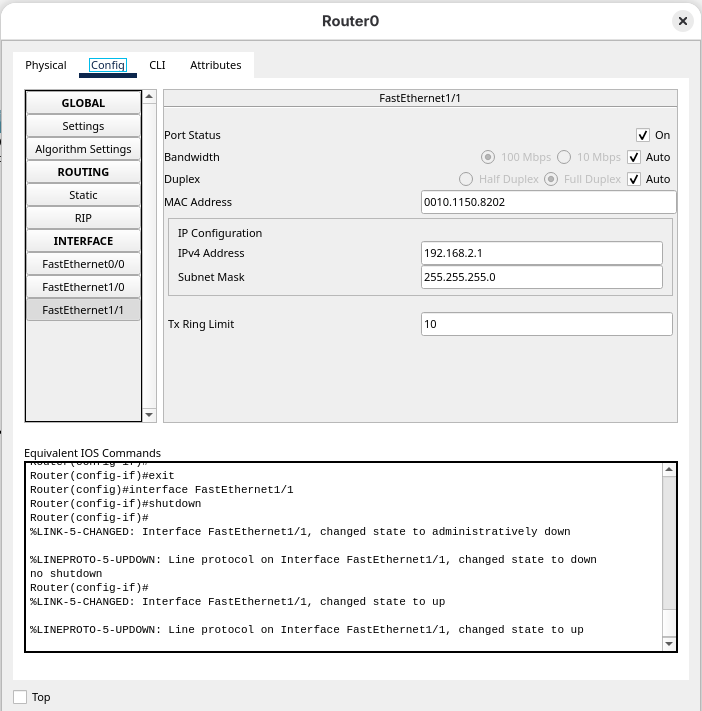
\includegraphics[width=1\textwidth]{img/4.png}
\end{figure}
و بعد از پیکربندی اتصال بین اجزا ایجاد می‌شود.
\begin{figure}[h]
    \centering
    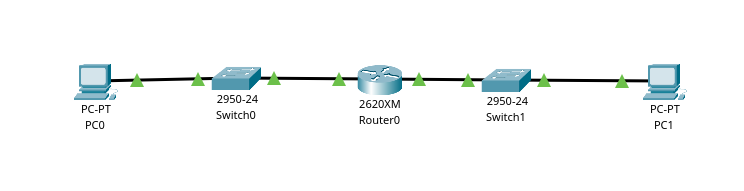
\includegraphics[width=1\textwidth]{img/5.png}
\end{figure}

\clearpage
جال باید کامپیوترها را نیز کانفیگ کنیم پس مانند قبل در تب \lr{config} ابتدا پیکربندی لازم را برای دستگاه انجام داده و بعد \lr{FastEthernet0} را تنظیم می‌کنیم.
\begin{figure}[h]
    \centering
    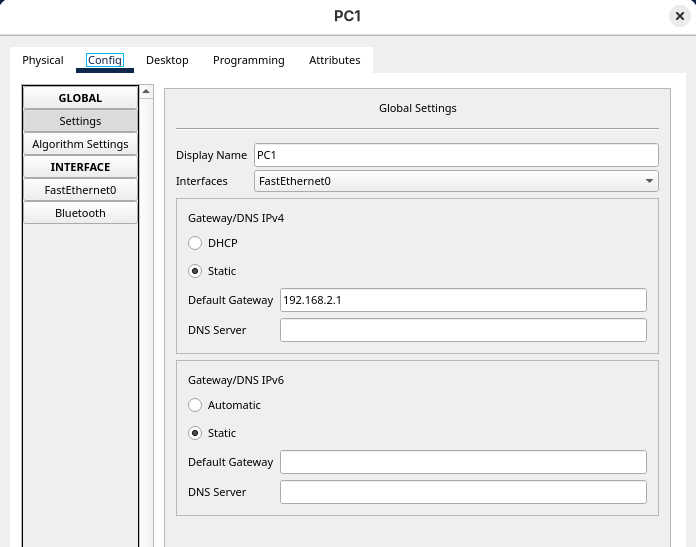
\includegraphics[width=0.70\textwidth]{img/6.png}
    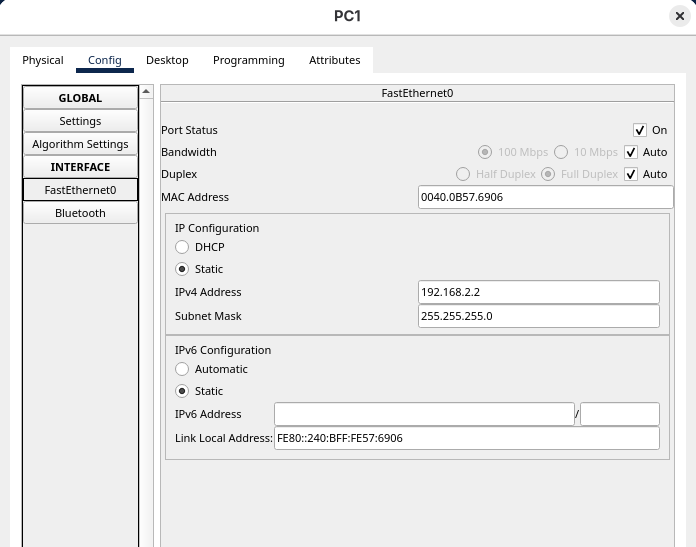
\includegraphics[width=0.8\textwidth]{img/7.png}
\end{figure}
\begin{figure}[h]
    \centering
\end{figure}
\begin{figure}[h]
    \centering
    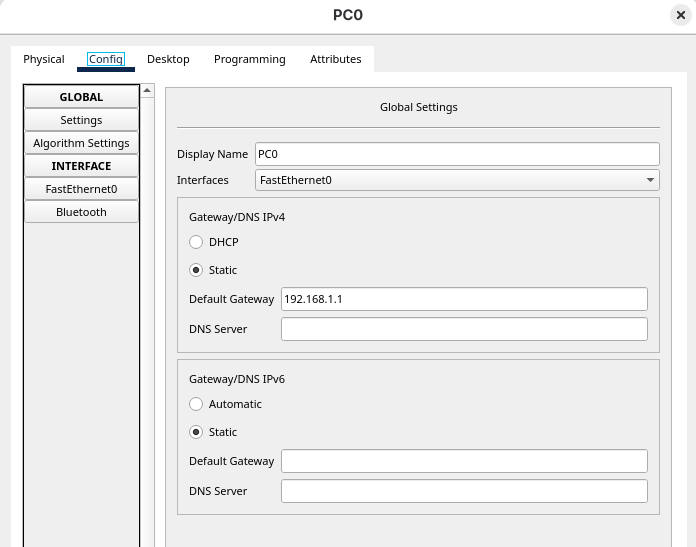
\includegraphics[width=0.8\textwidth]{img/8.png}
    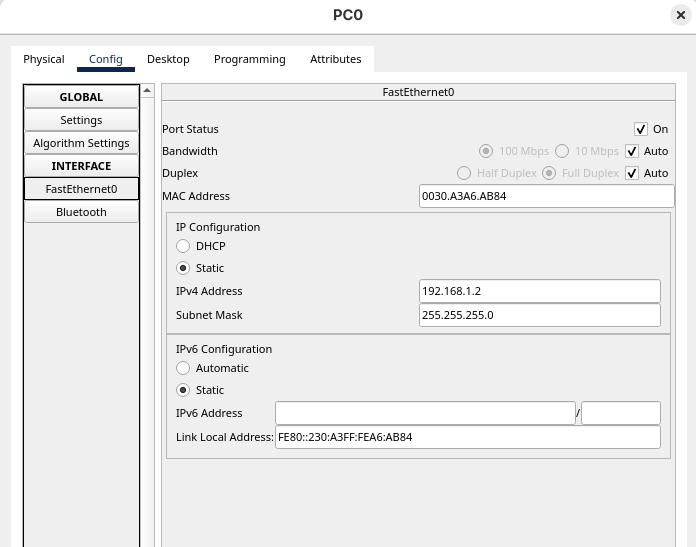
\includegraphics[width=0.8\textwidth]{img/9.png}
\end{figure}

\clearpage
برای تست کردن در کامپیوتر سمت چپ در بخش \lr{Desktop} در \lr{‫‪Command‬‬ Prompt‬‬} به کامپیوتر سمت راست پینگ می‌زنیم.

\begin{figure}[h]
    \centering
    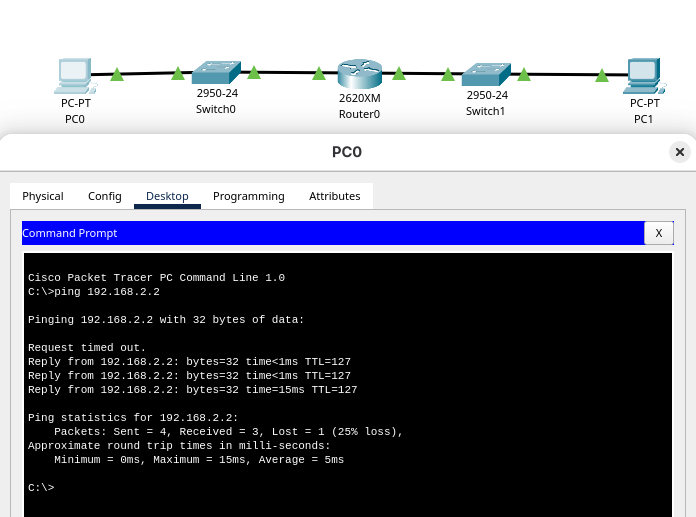
\includegraphics[width=1\textwidth]{img/10.png}
\end{figure}
\clearpage


\subsectionaddtolist{طراحی سناریوی دوم}

مانند بخش قبل تمامی اجرا را با استفاده از کابل \lr{‫‪cooper straight-through‬‬‬} به هم وصل می‌کنیم. اما در اتصال دو روتر به هم نیاز است که از کابل \lr{serial ‫‪DCE‬‬} استفاده شود پس با خاموش کردن روترها ماژول \lr{WIC-1T} را به آنها اضافه می‌کنیم. 
\begin{figure}[h]
    \centering
    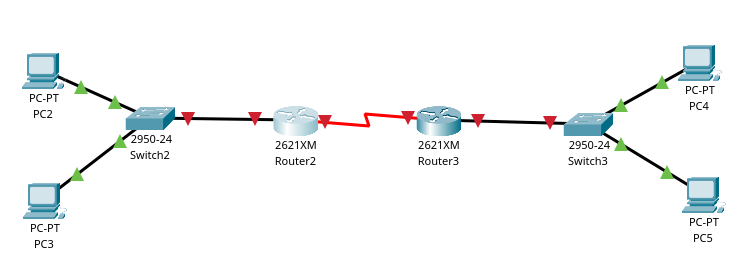
\includegraphics[width=1\textwidth]{img/12.png}
\end{figure}
\begin{figure}[h]
    \centering
    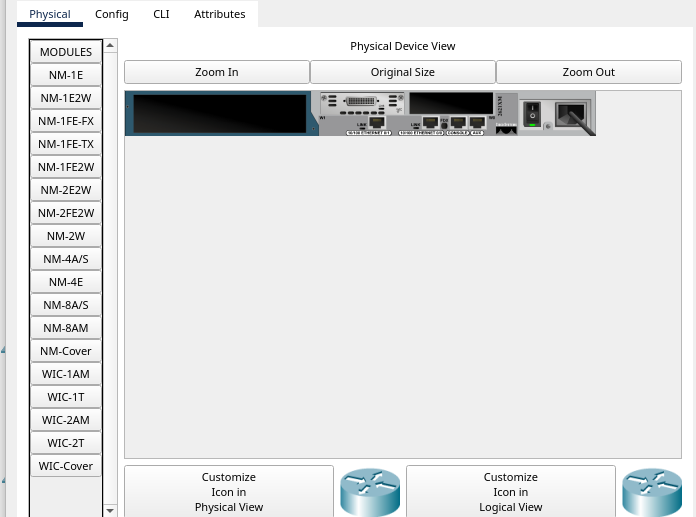
\includegraphics[width=1\textwidth]{img/11.png}
\end{figure}

برای اینکه اتصال بین دو روتر برقرار شود باید طبق فیلم با کلیک بر روی روترها در بخش config و در \lr{serial 0/0} مقدار کلاک را به 56000 تغییر دهیم و گزینه on را فعال کنیم.
\begin{figure}[h]
    \centering
    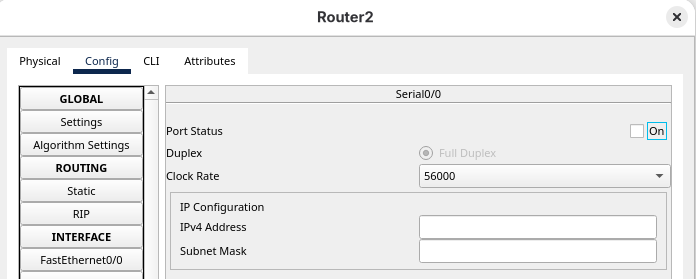
\includegraphics[width=1\textwidth]{img/14.png}
    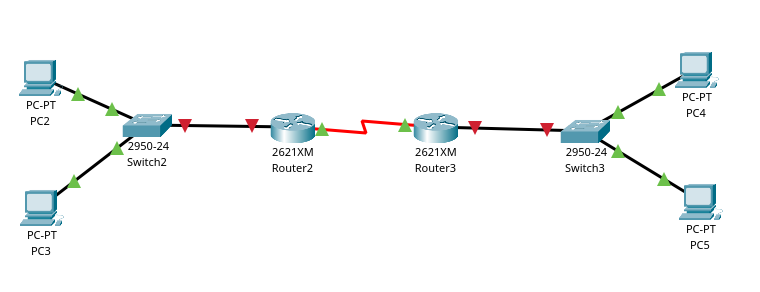
\includegraphics[width=1\textwidth]{img/13.png}
\end{figure}
\clearpage
حال مانند بخش قبل به پیکربندی اجزا می‌پردازیم.

\begin{figure}[h]
    \centering
    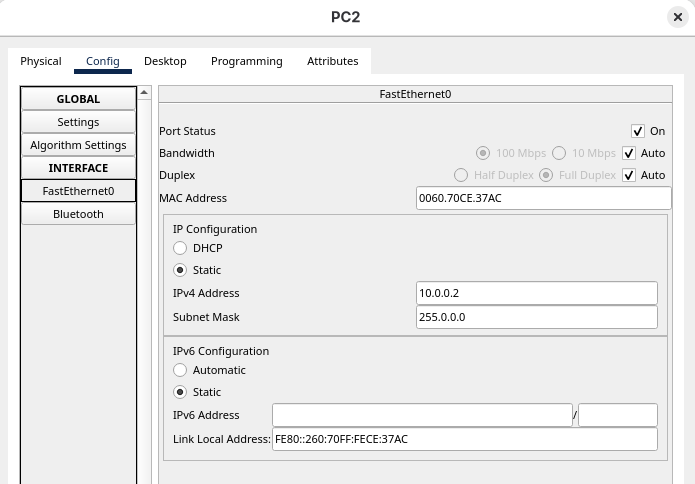
\includegraphics[width=1\textwidth]{img/15.png}
\end{figure}
\begin{figure}[h]
    \centering
    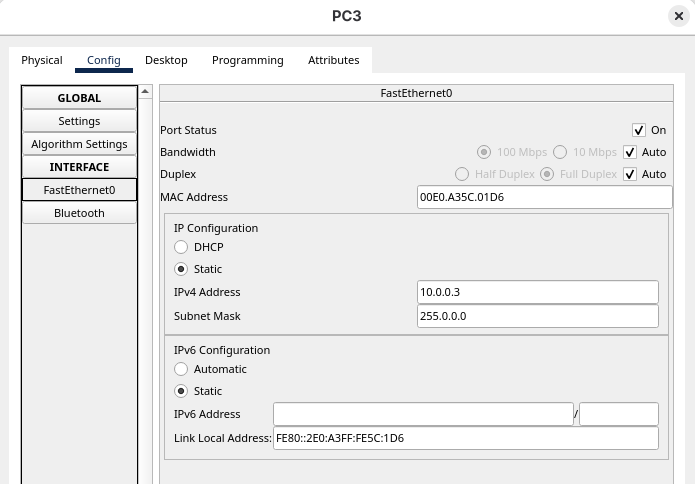
\includegraphics[width=1\textwidth]{img/16.png}
\end{figure}
\begin{figure}[h]
    \centering
    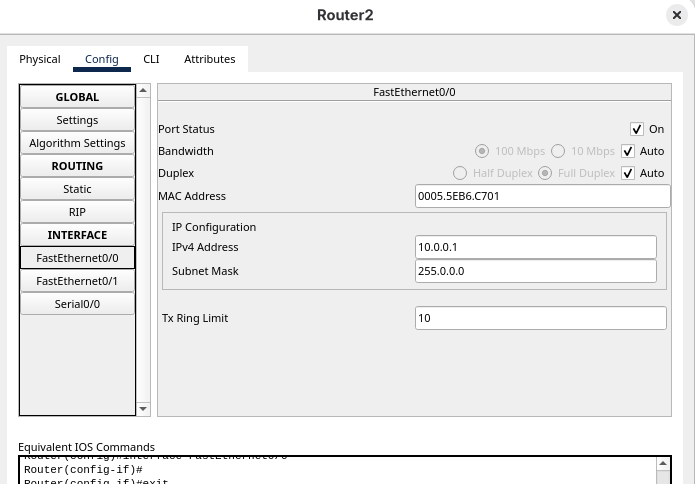
\includegraphics[width=1\textwidth]{img/17.png}
\end{figure}
\begin{figure}[h]
    \centering
    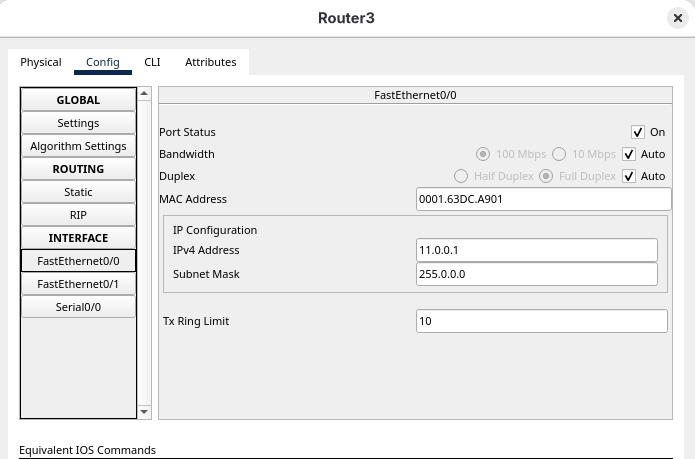
\includegraphics[width=1\textwidth]{img/18.png}
\end{figure}
\begin{figure}[h]
    \centering
    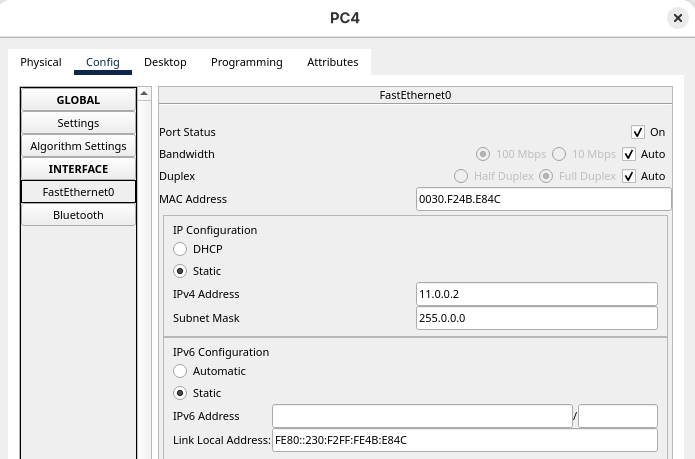
\includegraphics[width=1\textwidth]{img/19.png}
\end{figure}
\begin{figure}[h]
    \centering
    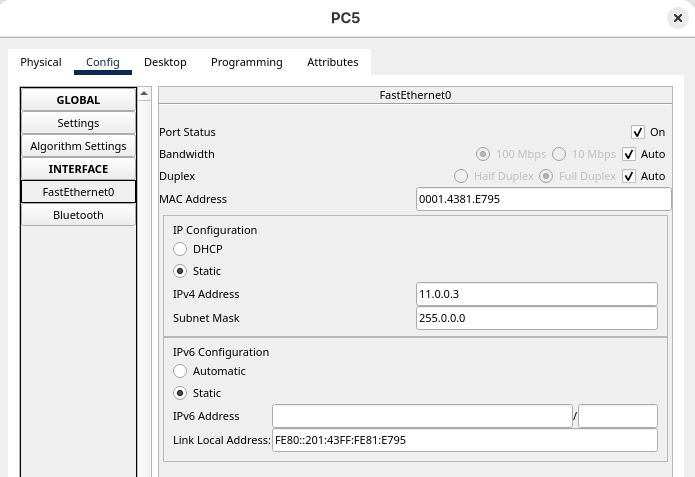
\includegraphics[width=1\textwidth]{img/20.png}
\end{figure}
\begin{figure}[h]
    \centering
    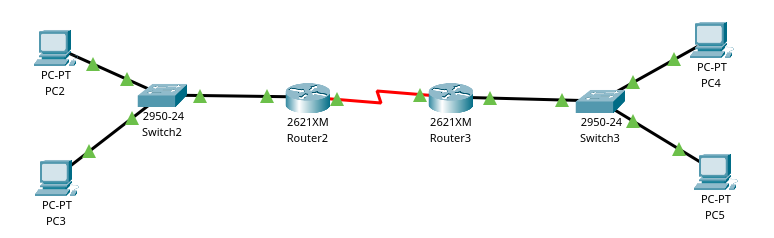
\includegraphics[width=1\textwidth]{img/21.png}
\end{figure}

\clearpage
تا الان اتصال بین کامپیوترها با سوئیچ مشترک برقرار است اما طبق فیلم برای اینکه روترها را هم بشناسیم باید یک subnet بین آنها تعریف شود. 
\begin{figure}[h]
    \centering
    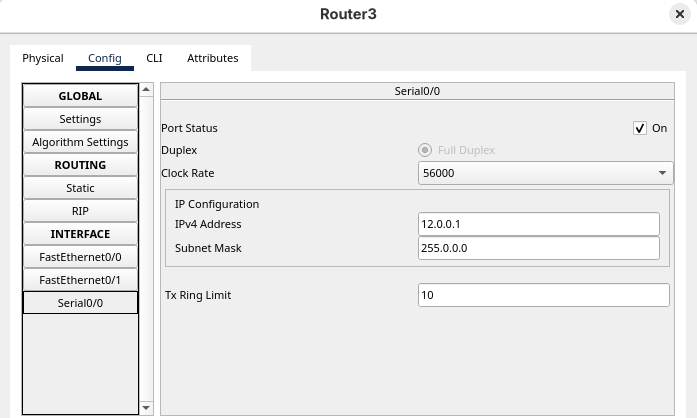
\includegraphics[width=1\textwidth]{img/22.png}
\end{figure}
\begin{figure}[h]
    \centering
    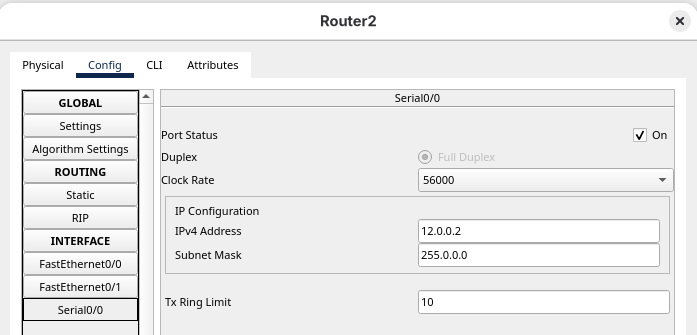
\includegraphics[width=1\textwidth]{img/23.png}
\end{figure}
\\
حال باید روترها بتوانند subnet دیگری را از طریق لینک داده شده عبور دهد. برای اینکار در بخش config در منوی static آی‌پی‌های مجاز را وارد می‌کنیم.
\begin{figure}[h]
    \centering
    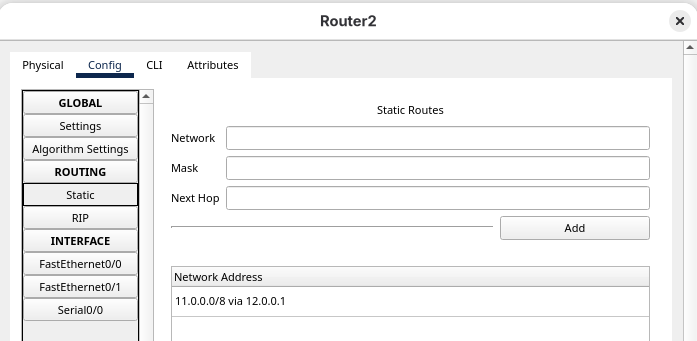
\includegraphics[width=1\textwidth]{img/26.png}
    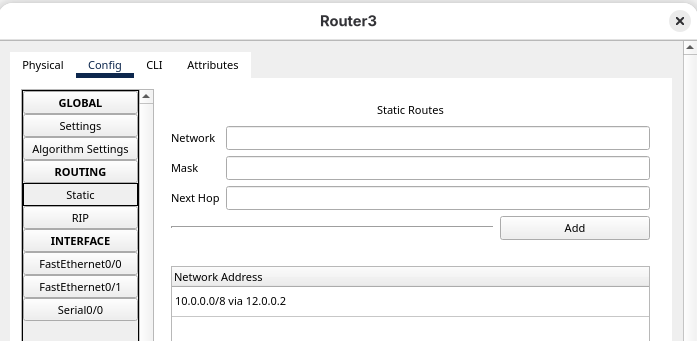
\includegraphics[width=1\textwidth]{img/27.png}
\end{figure}

\clearpage
برای تست مانند بخش قبل بین کامپیوترها از دستور پینگ استفاده می‌کنیم.
\begin{figure}[h]
    \centering
    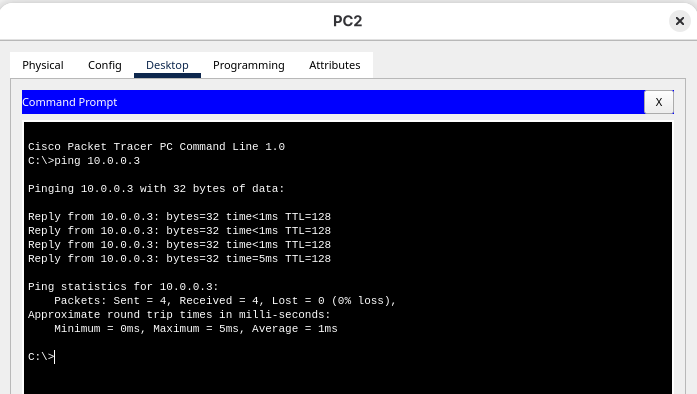
\includegraphics[width=1\textwidth]{img/24.png}
    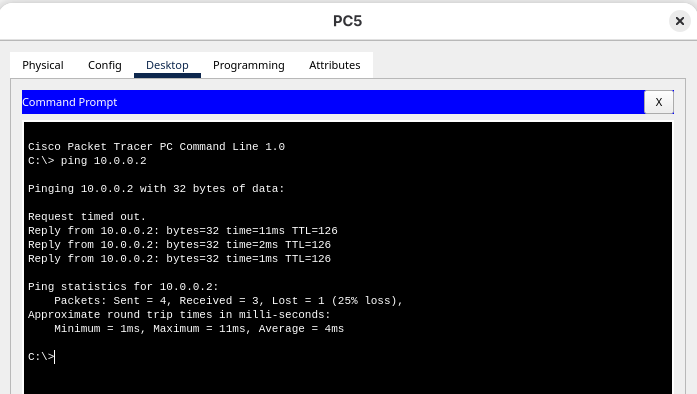
\includegraphics[width=1\textwidth]{img/25.png}
\end{figure}


\clearpage

\subsectionaddtolist{سوالات}

\textbf{با انتخاب سوئیچ در CLI و وارد کردن ؟}
\\
اینکار باعث نمایش دستورات و توضیحات آنها می‌شود.
\begin{figure}[h]
    \centering
    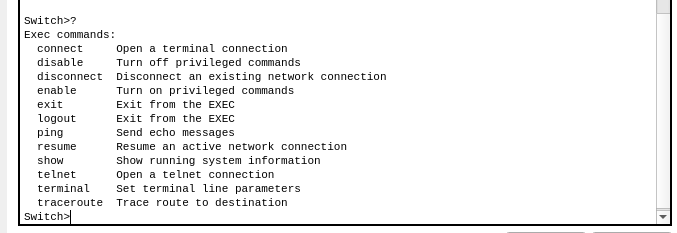
\includegraphics[width=1\textwidth]{img/q/1.png}
\end{figure}

\\
\textbf{عملکرد دستورات}
\\
سوئیچ‌های شبکه، به‌ویژه سوئیچ‌های برند سیسکو، دارای سطوح مختلفی از دسترسی در محیط خط فرمان (CLI) هستند. یکی از این سطوح، \lr{User EXEC Mode} است که پایین‌ترین سطح دسترسی محسوب می‌شود.
\lr{User EXEC Mode} اولین سطحی است که پس از اتصال به سوئیچ از طریق کنسول، Telnet یا SSH وارد آن می‌شوید. این مود فقط اجازه اجرای برخی دستورات نمایشی یا بررسی محدود وضعیت دستگاه را می‌دهد و امکان اعمال تغییرات در پیکربندی سوئیچ را ندارد.برای اعمال تغییر در پیکربندی سوئیچ، نیاز به ورود به حالت \lr{Privileged EXEC} و سپس \lr{Configuration Mode} است.

\begin{itemize}
    \item \lr{enable}: ورود به حالت \lr{Privileged EXEC} برای دسترسی بیشتر
    \item \lr{exit}: خروج از جلسه ترمینال یا بازگشت به مرحله قبلی
    \item \lr{logout}: قطع کامل اتصال از سوئیچ
    \item \lr{ping [آدرس IP]}: ارسال پیام ICMP برای بررسی ارتباط شبکه با مقصد مشخص
    \item \lr{traceroute [آدرس IP]}: ردیابی مسیر بین سوئیچ و یک مقصد مشخص
    \item \lr{show version}: نمایش اطلاعات مربوط به نسخه سیستم‌عامل، سخت‌افزار و uptime دستگاه
    \item \lr{show interfaces}: مشاهده وضعیت فعلی تمام رابط‌های شبکه (interfaces)
    \item \lr{show ip interface brief}: نمایش خلاصه‌ای از وضعیت و پیکربندی IP رابط‌ها
    \item \lr{show mac address-table}: مشاهده جدول نگاشت آدرس‌های MAC شناخته‌شده توسط سوئیچ
    \item \lr{show arp}: نمایش جدول ARP ،نگاشت آدرس‌های IP به MAC
    \item \lr{show history}: مشاهده لیست دستورات وارد شده در نشست جاری
    \item \lr{terminal length}: تعیین تعداد خطوطی که در هر صفحه خروجی CLI نمایش داده می‌شود
    \item \lr{ping ipv6 [آدرس IPv6]}: ارسال پینگ به مقصد دارای آدرس \lr{IPv6}
    \item \lr{traceroute ipv6 [آدرس IPv6]}: ردیابی مسیر ترافیک به مقصد با آدرس \lr{IPv6}
\end{itemize}


\clearpage
\textbf{اجرای دستورات show}
\\
\begin{figure}[h]
    \centering
    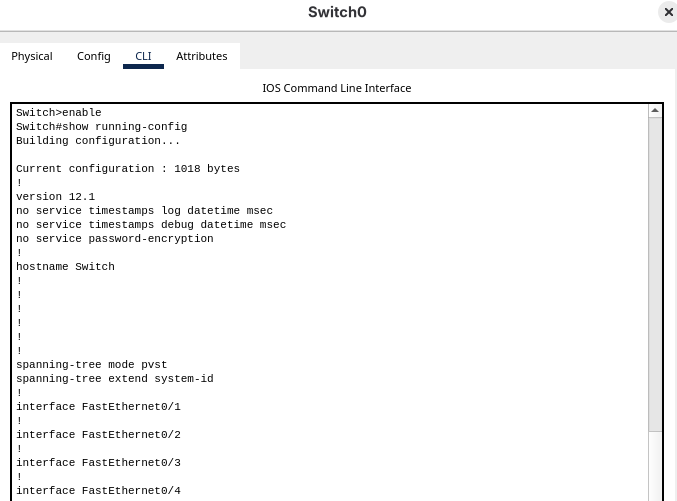
\includegraphics[width=1\textwidth]{img/q/2.png}
\end{figure}
\lr{show running-config}: این دستور تنظیمات روتر و سوئیچ را نمایش می‌دهد.
\\
\begin{figure}[h]
    \centering
    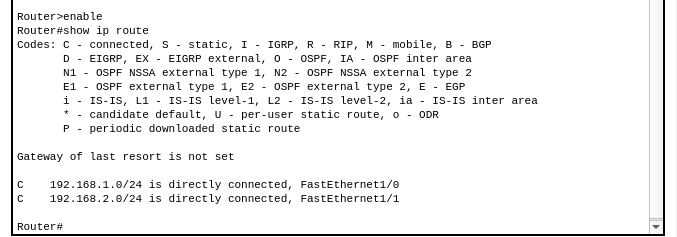
\includegraphics[width=1\textwidth]{img/q/3.png}
\end{figure}
\lr{show ip route}: این دستور فقط برای روتر است و IPهای تنظیم شده بر روی interfaceهای مختلف را نمایش می‌دهد. 
\\
\begin{figure}[h]
    \centering
    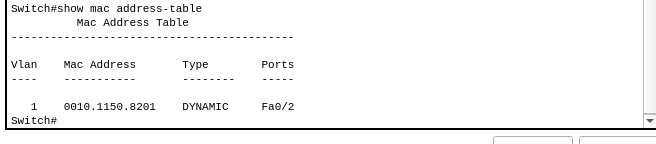
\includegraphics[width=1\textwidth]{img/q/4.png}
\end{figure}
\lr{show mac address-table}: این دستور برای سوئیچ است و آدرس mac دستگاه‌های متصل به سوئیچ را و پورت آن را نمایش می‌دهد. این جدول در هنگام پینگ گرفتن پر می‌شود.
\\
\begin{figure}[h]
    \centering
    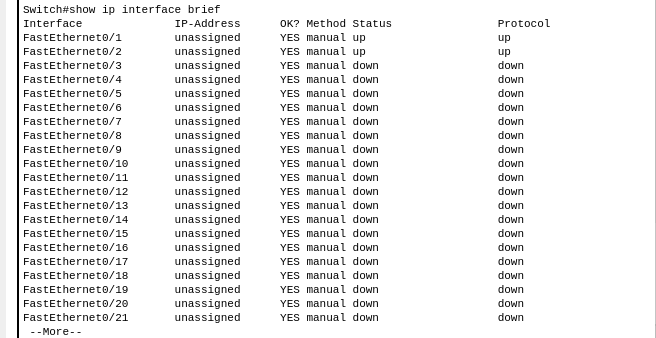
\includegraphics[width=1\textwidth]{img/q/5.png}
\end{figure}
\lr{show ip interface brief}: این دستور \lr{IP address}های مختبف interfaceها را نمایش می‌دهد. و برای سوئیچ و روتر کاربرد دارد.
\\
\begin{figure}[h]
    \centering
    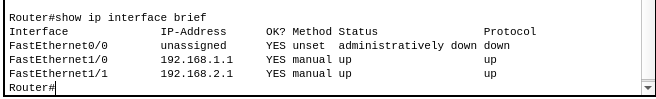
\includegraphics[width=1\textwidth]{img/q/6.png}
\end{figure}
\lr{show vlan brief}: این دستور اطلاعاتی درباره‌ی vlanها می‌دهد و برای سوئیچ قابل اجرا است.
\\
\begin{figure}[h]
    \centering
    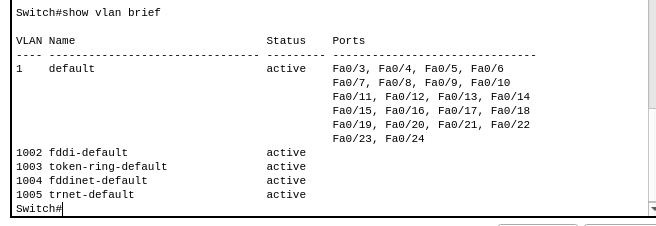
\includegraphics[width=1\textwidth]{img/q/7.png}
\end{figure}

\clearpage
\textbf{gateway}

دروازه پیش‌فرض، دستگاهی در یک شبکه کامپیوتری است که ترافیک شبکه را از یک شبکه به شبکه دیگر هدایت می‌کند. این دستگاه در اکثر شبکه‌ها همان روتر است.
زمانی‌که یک دستگاه (مانند کامپیوتر یا سوئیچ) بخواهد با دستگاهی در خارج از شبکه محلی (LAN) خود ارتباط برقرار کند، بسته‌های اطلاعاتی را به Gateway ارسال می‌کند. Gateway پس از دریافت بسته‌ها، آن‌ها را به مقصد مناسب در شبکه دیگر هدایت می‌کند.
 کاربرد های Gateway :
ایجاد امکان ارتباط بین شبکه‌های محلی مختلف
مسیریابی بسته‌های داده به سمت شبکه‌های دیگر یا اینترنت
کنترل و فیلتر کردن ترافیک ورودی و خروجی
اجرای سیاست‌های امنیتی یا مسیریابی در سطح شبکه

برای مثال اگر کامپیوتری در شبکه‌ای با \lr{IP 192.168.1.10} و \lr{Subnet Mask 255.255.255.0} بخواهد با سروری با \lr{IP 8.8.8.8} ارتباط برقرار کند، ابتدا تشخیص می‌دهد که مقصد در شبکه محلی نیست و بسته را به Gateway، مثلاً \lr{192.168.1.1}، ارسال می‌کند. Gateway این بسته را دریافت کرده و به سمت مقصد هدایت می‌کند.


\clearpage

\end{document}